\chapter{Phase shift transducer}
\section{Theory and related work} \label{sec:literature_phasetransducer}
This circuit comprises the use of voltage comparators used as zero crossing detectors, a XOR gate as well as a low pass filter. An operational amplifier comparator is a circuit that compares one analogue voltage level with a reference voltage and outputs a signal based on this voltage comparison, this operational amplifier is used in open loop mode and switches between its two saturated states \cite{OpAmpComparator}.\vspace{4mm} \newline 
A XOR gate is a digital logic gate with two or more inputs and one output and performs the exclusive disjunction between these input voltage levels \cite{XORGate}.
A low pass filter is a circuit that allows signals with a frequency lower than that of the cut-off frequency to pass through it, and blocks all frequencies higher than the cut off frequency. A single pole low pass filter consisting of a resistor and a capacitor can be used to smooth a PWM signal into an analogue voltage level \cite{PWMref}.

\section{Design} \label{sec:design_phasetransducer}
The first step in determining the phase difference between two sinusoidal waves is to determine when each of these sinusoidal signals pass through the zero axis, and more specifically when each sinusoid is positive. This was implemented by using an operational amplifier comparator as a zero crossing detector, in this configuration the input voltage was applied at the non inverting pin and the reference input was applied at the inverting input pin and was set to \SI{100}{\milli \volt} \cite{ZeroCrossingDetector}. It was found that a ground reference produced an unstable and unpredictable output due to noise under no load conditions, the design was then changed to use a very small reference voltage for the comparator. These individual \SI{100}{\milli \volt} reference signals were implemented by using a voltage divider circuit, by selecting $R_1$ as a $100k\Omega$ resistor a value for $R_2$ could be found as $1.995k\Omega$. These second resistors were implemented using a potentiometer so that the PWM output of the comparators could be calibrated under no load conditions as to provide a more accurate output. The operational amplifier used for this design was the TLC2272, this chip was chosen due to its rail to rail capabilities and due to space constraints as it contained two operational amplifiers per chip. Both of the comparators were used in single supply mode, thus its two saturated states corresponded to \SI{0}{\volt} and \SI{5}{\volt} respectively, this meant that if an input signal was positive the comparator's output would be \SI{5}{\volt}, and if the signal was less than the reference signal the output would be \SI{0}{\volt}. \vspace{4mm} \newline
The input voltage to the zero crossing detector for the voltage level was taken as the output from the voltage divider network in Figure \ref{fig:voltagepeakdetector.pdf}, labelled as $v_{meas}$, and the input voltage to the zero crossing detector for the current level was taken as the output from the gain stage in Figure \ref{fig:currentpeakdetector.pdf}, labelled as $i_{meas}$. Both of these input signals had a maximum voltage of \SI{5}{\volt} and thus were within the limits of the differential mode input of the operational amplifiers. Given that it was now determined when each sinusoidal input crossed the zero axis the phase delay between these signals could now be found. This was done by using a XOR gate that would output a logical high for the duration that the two sinusoids were out of phase \cite{PWMref}. This XOR gate was implemented by using a CD4070B integrated chip, where this integrated chips rail voltages had to be supplied by the \SI{5}{\volt} rail and ground respectively \cite{CD4070B:2003}. \vspace{4mm} \newline
As the inputs of the XOR gate are periodic square wave signals, the output would be a square wave pulse train with varying duty cycle dependant on how out of phase the input signals are, thus the frequency domain equivalent of this circuit would be a series of dirac deltas at multiples of the fundamental frequency enveloped by a sinc function. To turn this PWM signal into an analogue signal a crude digital to analogue converter was implemented by using a single pole RC low pass filter to filter out all of the dirac deltas in the frequency domain \cite{PWMref}. The components of the low pass filter were selected using Equation \ref{eq:cutofffreqcap} and choosing a cut off frequency of 10Hz, where a fixed \SI{20}{\micro F} was selected and the resistor was implemented using a $\SI{56}{\kilo \Omega}$ potentiometer. This potentiometer was tuned until an output signal with an acceptable voltage ripple was obtained. As the output of this transducer had to be as accurate as possible all noise levels had to be kept to a minimum, thus all noise levels had to be as small as possible. This was achieved by implementing the smoothing capacitor at the output as two \SI{10}{\micro F} low ESR capacitors placed in parallel. Decoupling capacitors were also placed at the positive rails of the TLC2272 and the CD4070B to minimize the effects of the rail voltage noise on the output.
\begin{align}
    f_{cut-off}=\frac{1}{2\pi RC} 
   \label{eq:cutofffreqcap}
\end{align}
The transducer can measure a phase angle difference of up to $180^o$, which corresponds to a DC output voltage of \SI{5}{\volt}, Equation \ref{eq:angle_calc} had to be applied to convert the output DC voltage level to an angle in degrees. As the Arduino had a resolution of 10 bits the input signal could be measured with an accuracy of up to \SI{4.888}{\milli V}, this was equal to an angle of $0.176^o$ per bit.

\begin{align}
    V_{meas} =\frac{\phi_{load}}{180^o} 5
   \label{eq:angle_calc}
\end{align}

\begin{figure}[h!]
    \centering
    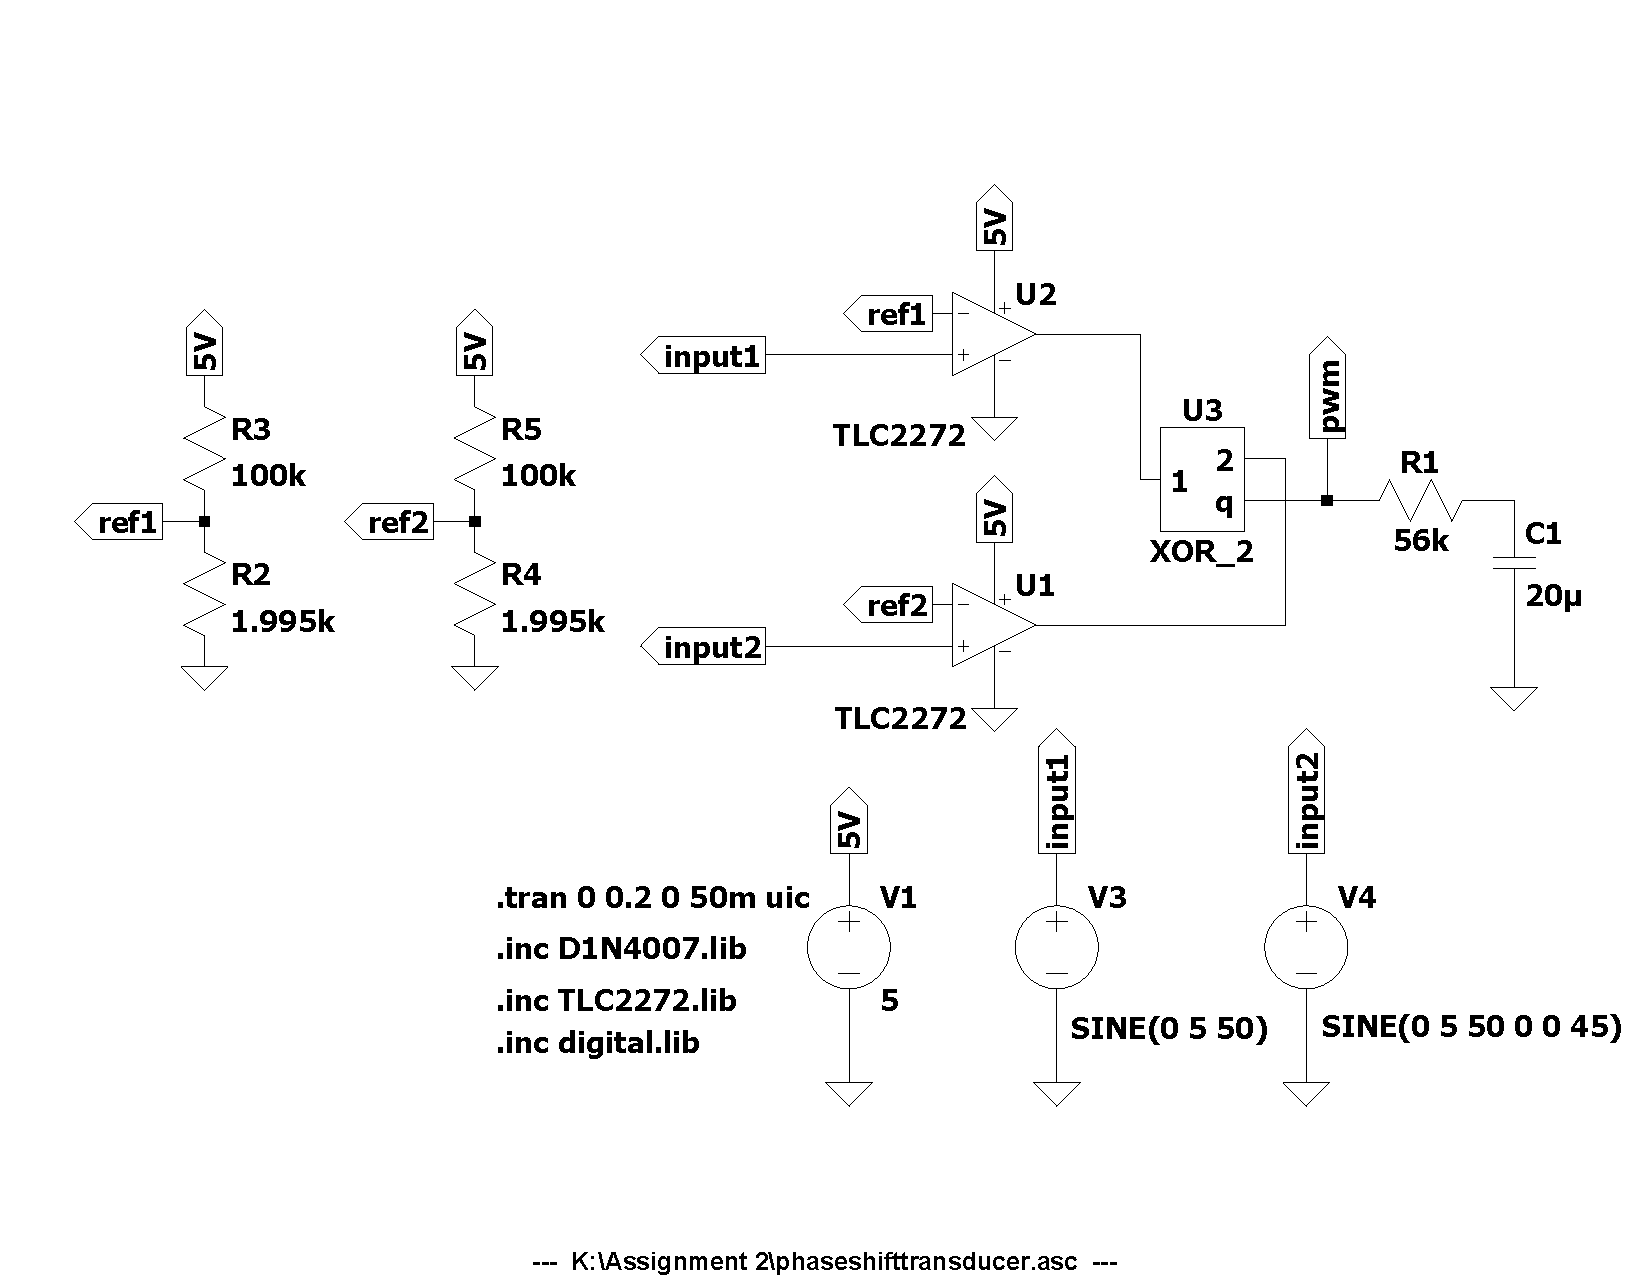
\includegraphics[width = 0.65\linewidth]{Figures/phaseshifttransducer.pdf}
        \caption{Phase Shift Detector Diagram}
    \label{fig:phaseshiftdetector.pdf}
\end{figure}

\section{Simulation} \label{sec:simulation_phasetransducer}
The phase transducer was tested in simulation by applying two out of phase sinusoidal signals at the inputs of the comparators and plotting the output PWM signal as well as the corresponding output DC voltage level. Given a load of 1k and $\SI{22}{\mu F}$ the output voltage was found to be 226mV, this is shown in Figure \ref{subfig:phasetransducer1k22uout}, with the corresponding PWM signal shown in Figure \ref{subfig:phasetransducer1k22u}. The transducer was also simulated with a load of 1k and $\SI{33}{\mu F}$, where output voltage was found to be 151mV, this is shown in Figure \ref{subfig:phasetransducer1k33uout}. The corresponding PWM signal for this input is shown in Figure \ref{subfig:phasetransducer1k33u}. 

\begin{figure}[h!]
 \centering
     \begin{subfigure}[]{0.45\textwidth}
        \centering
         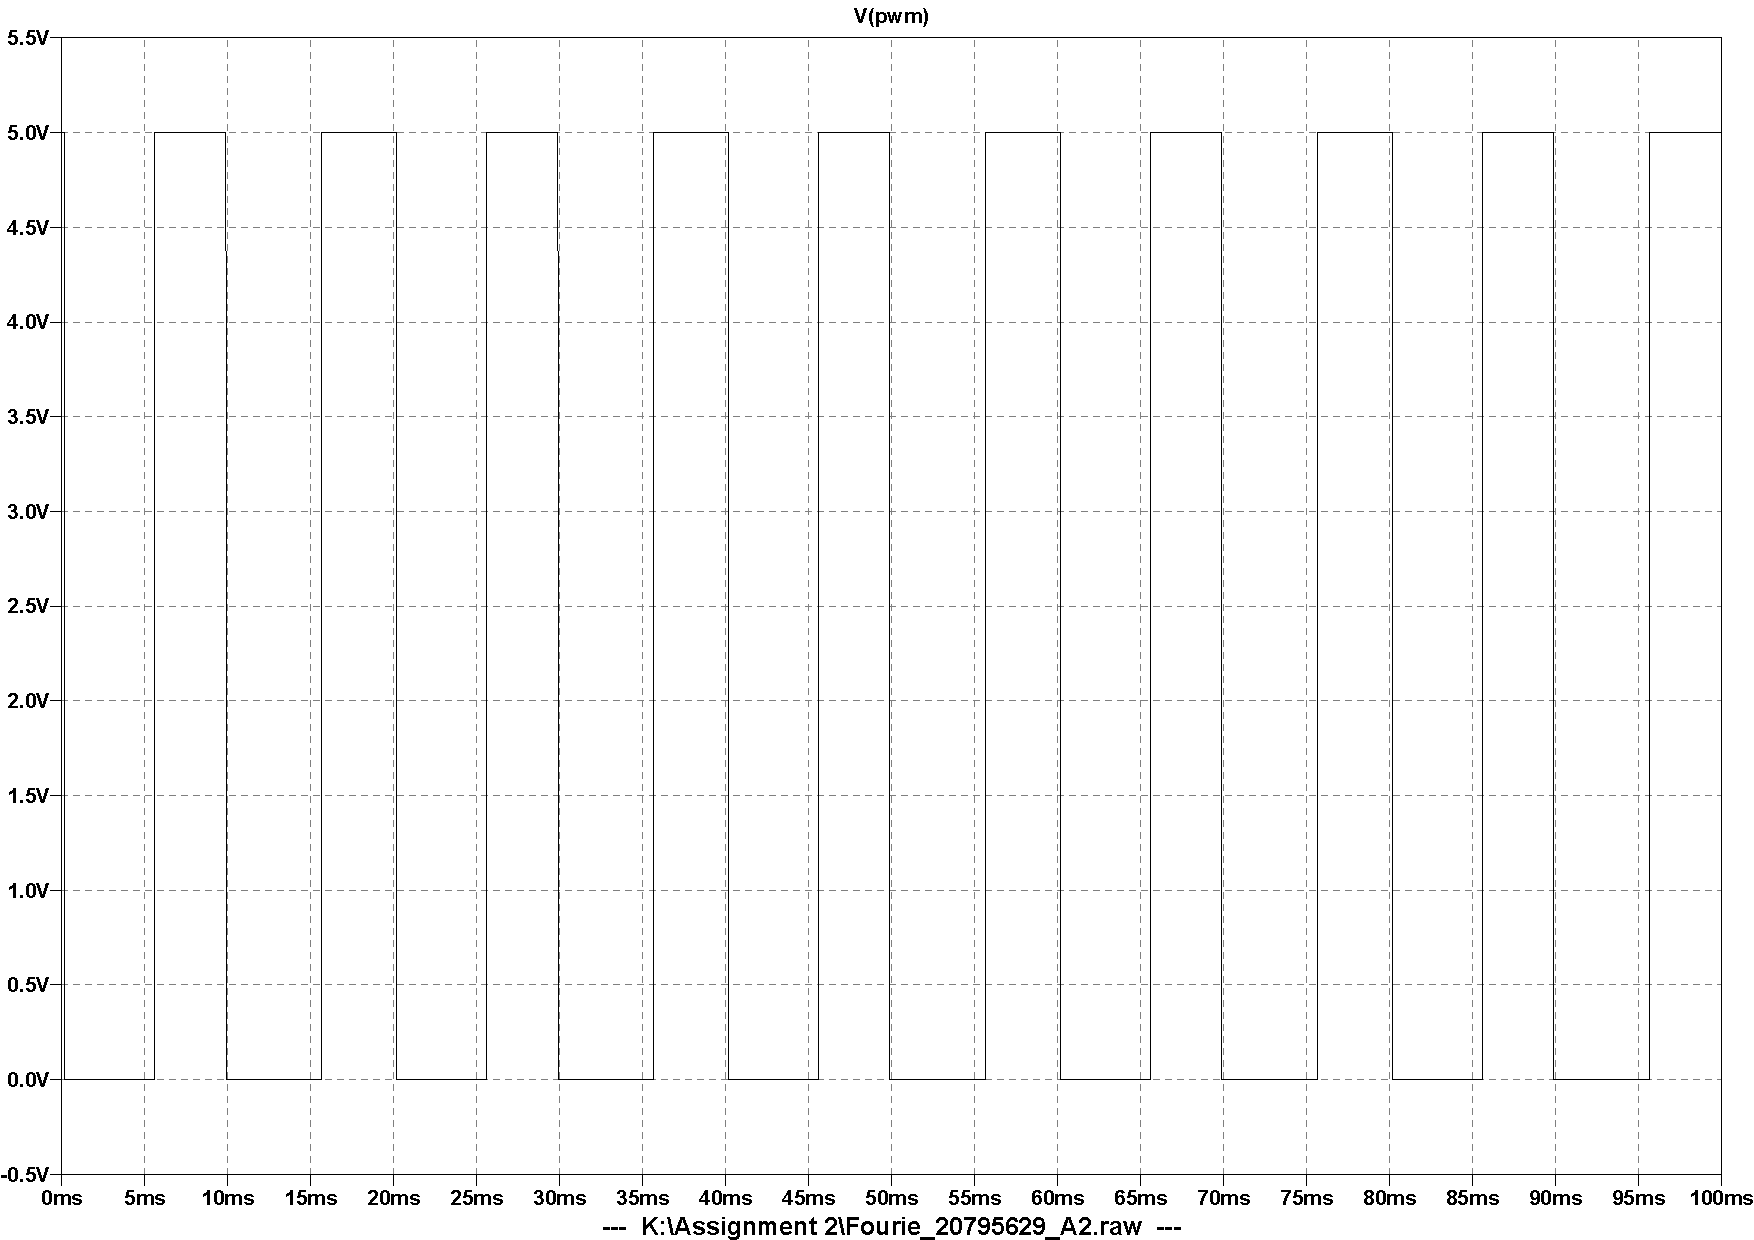
\includegraphics[width=1\linewidth]{./Figures/phasetransducer1k22u.pdf}
		    \caption{1k and $\SI{22}{\mu F}$ load PWM output} \label{subfig:phasetransducer1k22u}
     \end{subfigure}
     \begin{subfigure}[]{0.45\textwidth}
        \centering
         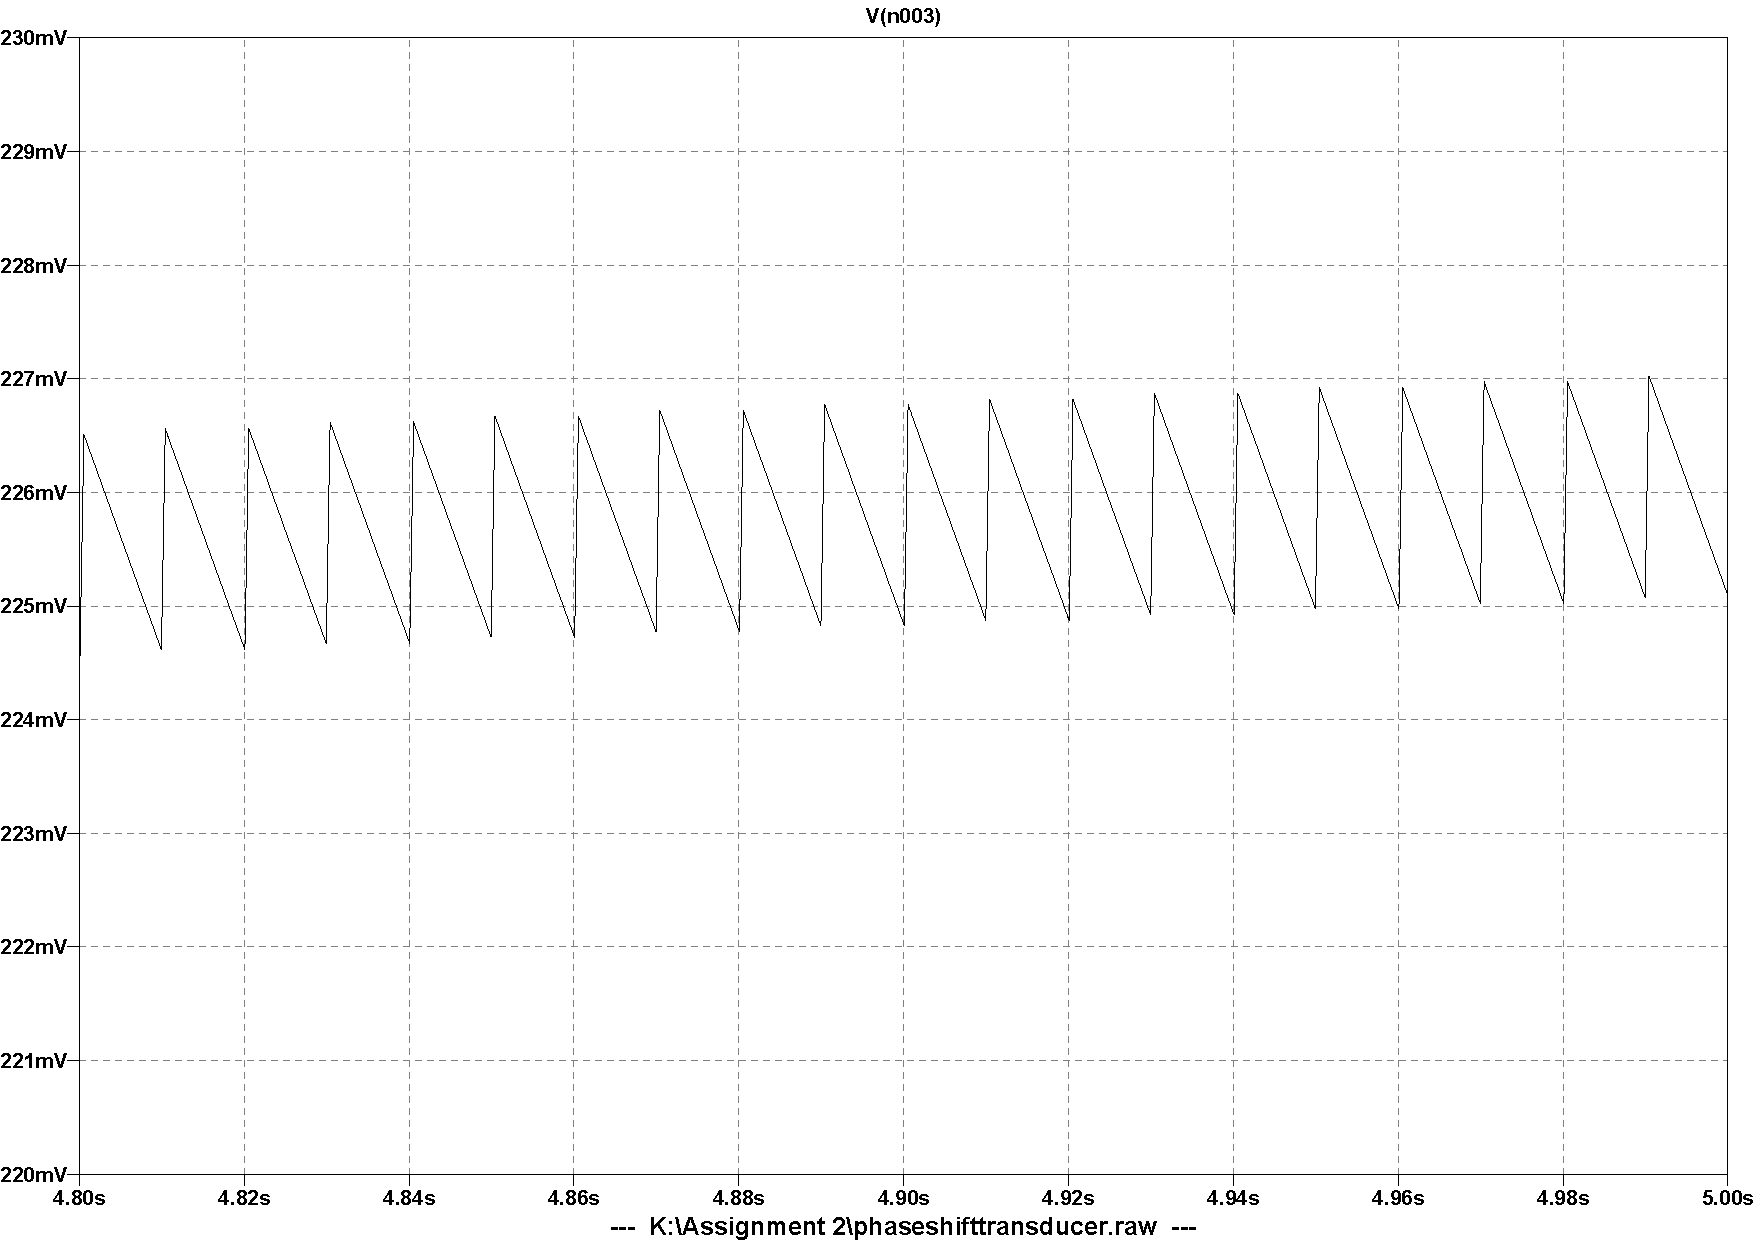
\includegraphics[width=1\linewidth]{./Figures/phaseshifttransducermidanalogout.pdf}
		    \caption{1k and $\SI{22}{\mu F}$ load DC output} \label{subfig:phasetransducer1k22uout}
     \end{subfigure}
   \caption[Simulated results for the phase transducer with a mid range load]{Output voltage ripple and response for the phase transducer with a mid range load of 1k and $\SI{22}{\mu F}$. (a) depicts PWM output signal, (b) depicts DC output signal. }
    \label{fig:simulation_results_box}
 \end{figure}
 
 \begin{figure}[h!]
 \centering
      \begin{subfigure}[]{0.45\textwidth}
              \centering
  		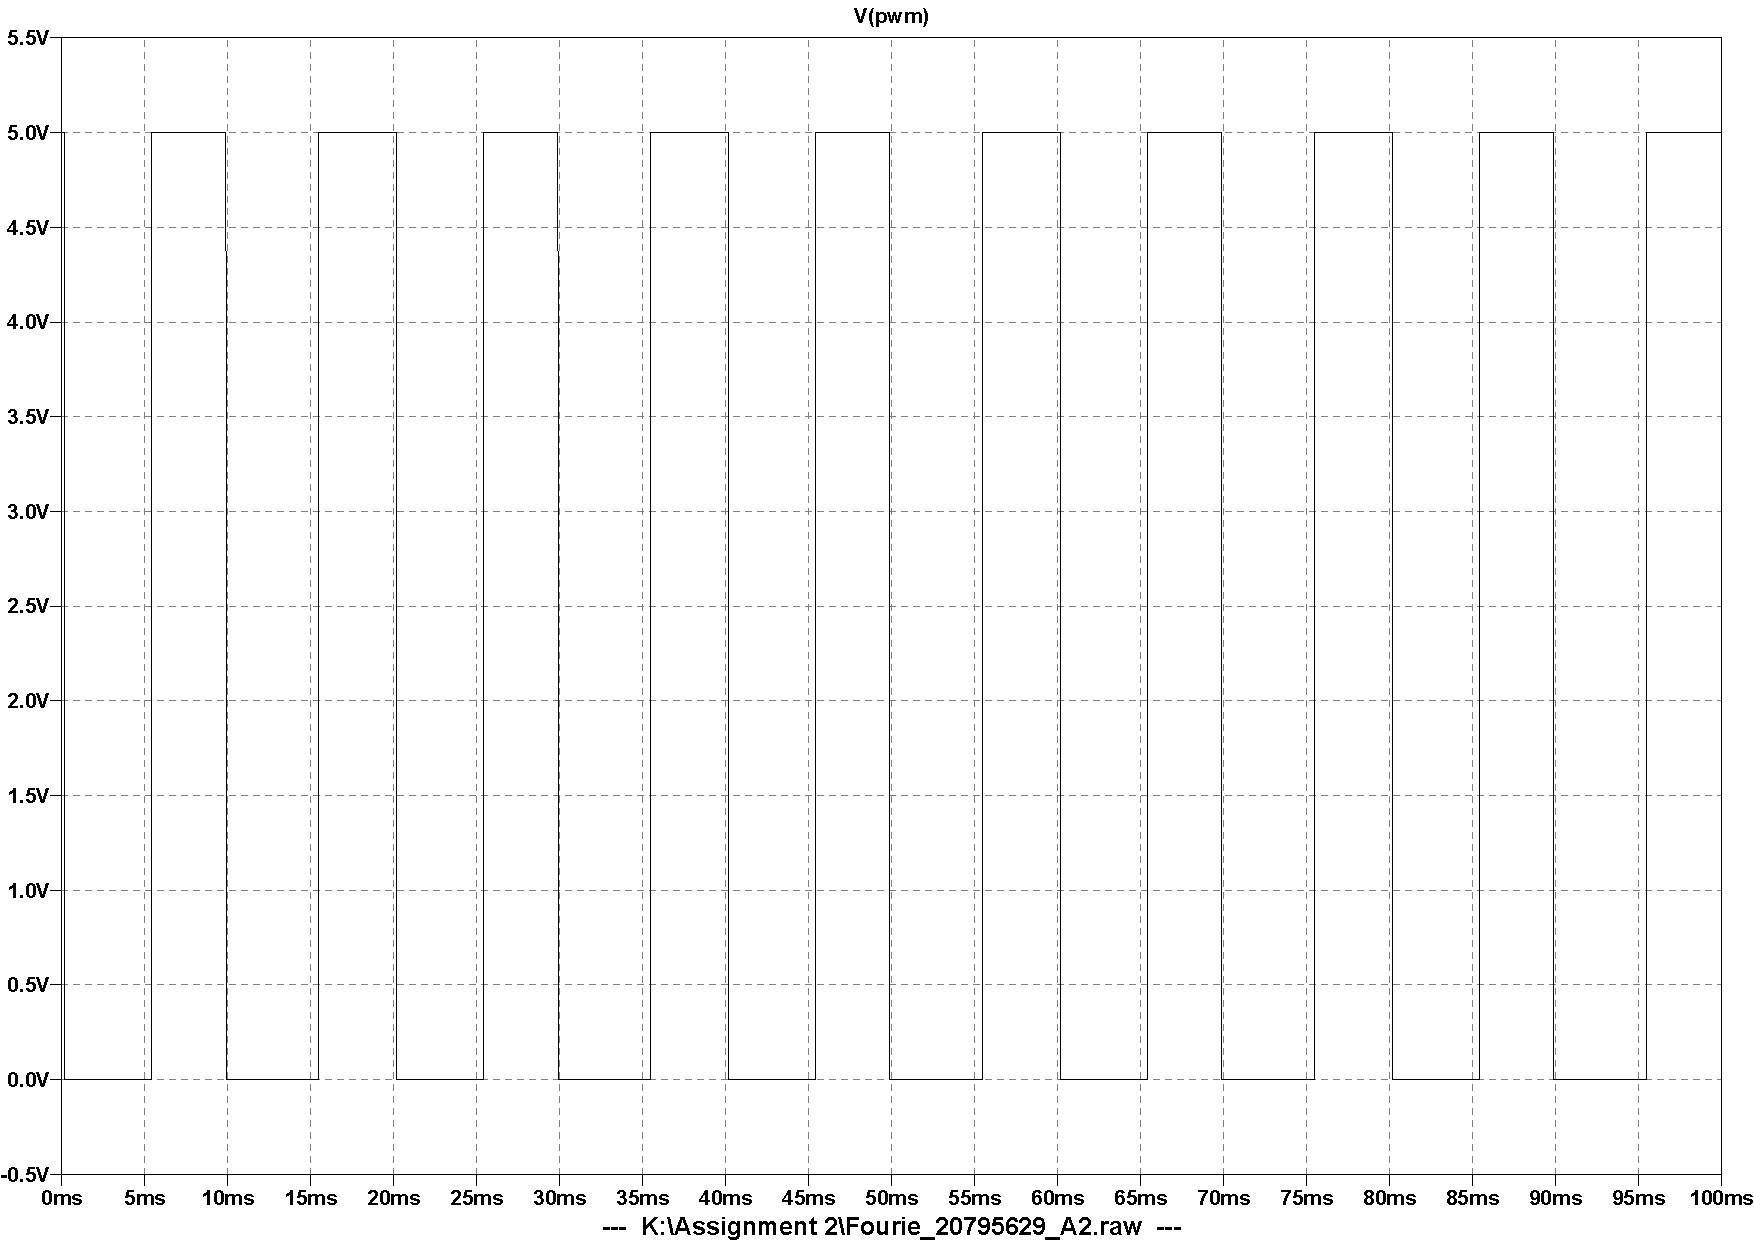
\includegraphics[width=1\linewidth]{./Figures/phasetransducer1k33u.pdf}
		    \caption{1k and $\SI{33}{\mu F}$ load PWM output} \label{subfig:phasetransducer1k33u}
     \end{subfigure}
     \begin{subfigure}[]{0.45\textwidth}
        \centering
         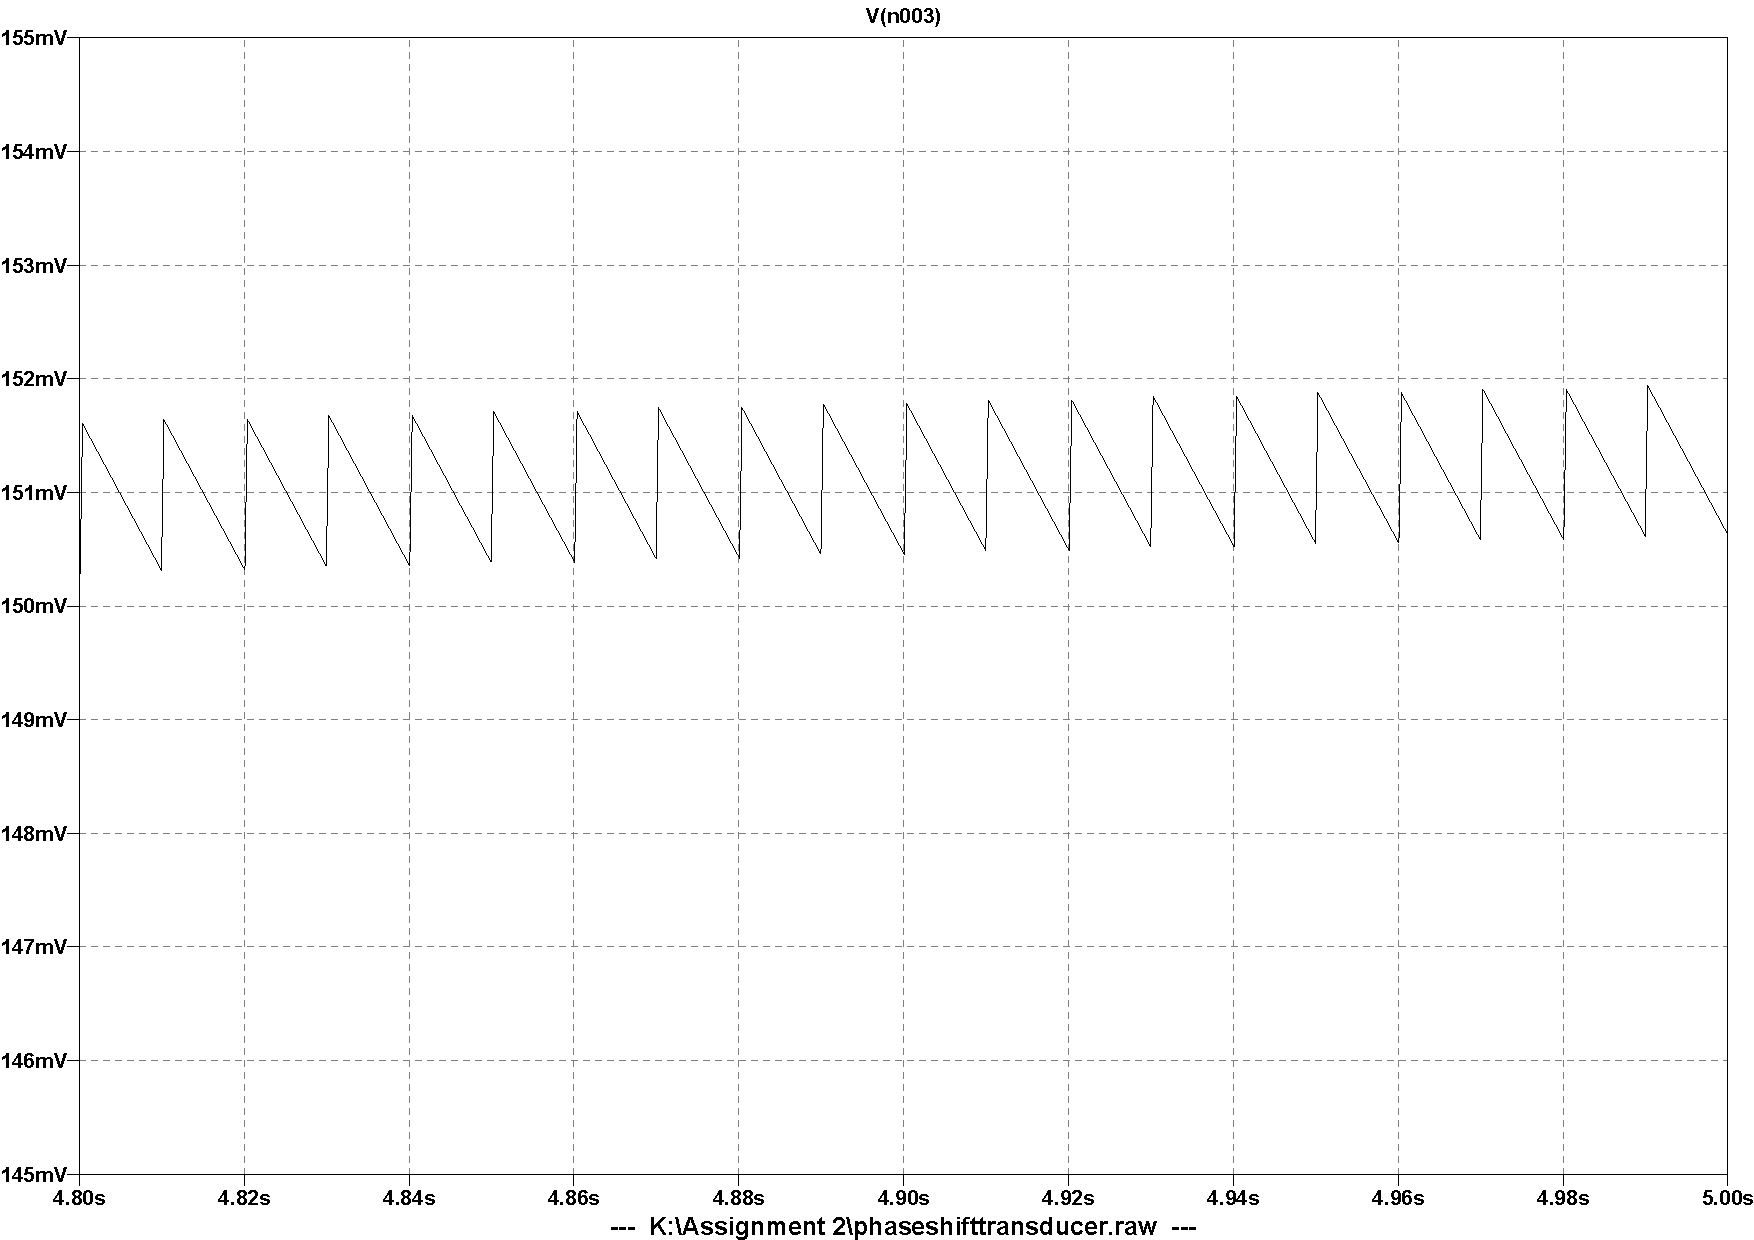
\includegraphics[width=1\linewidth]{./Figures/phaseshifttransducermiddanalogout.pdf}
		    \caption{1k and $\SI{33}{\mu F}$ load DC output} \label{subfig:phasetransducer1k33uout}
     \end{subfigure}
   \caption[Simulated results for the phase transducer with a mid range + $\delta$ load]{Output voltage ripple and response for the phase transducer with a mid range load of 1k and $\SI{33}{\mu F}$. (a) depicts PWM output signal, (b) depicts DC output signal. }
    \label{fig:simulation_results_box}
 \end{figure}

%\vspace{2mm} 
\section{Measurements} \label{sec:measurements_phasetransducer}
To test whether the phase transducer worked in practice integrated tests were performed using various loads as inputs as to induce different phase changes. The results of these measurements are tabulated in Table \ref{tab:phasetransducerrealtests}. Here the measured shift column refers to the average time difference between the voltage and current signals crossing the zero axis, and the applied shift refers to this average time shift converted to a phase angle. \vspace{4mm} \newline 
The output DC voltage level was related to the input phase angle by Equation \ref{eq:angle_calc}, and given these measurements it was found that the largest angle deviation was found to differ by $0.96^o$, which was within the tolerance of $1^o$. Figure \ref{subfig:phaseshifttransducermidrange} shows the oscilloscope measurement of the output of the phase transducer as PWM signal given a mid range input of 1k and $\SI{22}{\mu F}$. After passing this PWM signal through a low pass filter a DC signal was obtained, the ripple voltage associated with this DC signal is shown in Figure \ref{subfig:phaseshifttransducerripple}. Here it was found that the signal had a peak to peak voltage of only $\SI{15.6}{\milli V}$, and this result was less than the $\SI{27.78}{\milli V}$ accuracy required to ensure a measurement within $1^o$ of what was actually obtained.

\begin{table} [h!]
        \centering
        \scriptsize
        \caption{Phase shift transducer integrated test results.}
         \begin{tabular}{C{1.6cm} C{1.1cm} C{1.1cm} | C{2cm} C{1.8cm} C{1.8cm} C{1.5cm} C{1.5cm}}
           Measurement & Load R & Load C & Measured shift & Applied shift & Output level & Conversion & Difference\\
            & ($\Omega$) & ($\mu F$) & (ms) & ($^o$) & ($mV_{DC}$) & ($^o$) & ($^o$) \\
        \hline
            No shift      & 1k    & -   & 0.026 & 0.468 & 38.89  & 1.397  & 0.929 \\
            Max shift     & 1k    & 3.3 & 1.77 & 31.86 & 860.8  & 31.248  & 0.612 \\
            Mid range           & 1k    & 22  & 0.37& 6.66 & 197.6  & 7.11 & 0.45 \\
            Mid + $\delta$      & 1k    & 33 & 0.30 & 5.4 & 123.2 &4.44 & 0.96 \\
            Mid + $2\delta$     & 1k    & 47 & 0.18 & 3.24 & 77.6  & 2.78 & 0.46 \\
          \hline
        \end{tabular}
     \label{tab:phasetransducerrealtests}
\end{table}



\begin{figure}[h]
 \centering
    \begin{subfigure}[]{0.45\textwidth}
    \centering
             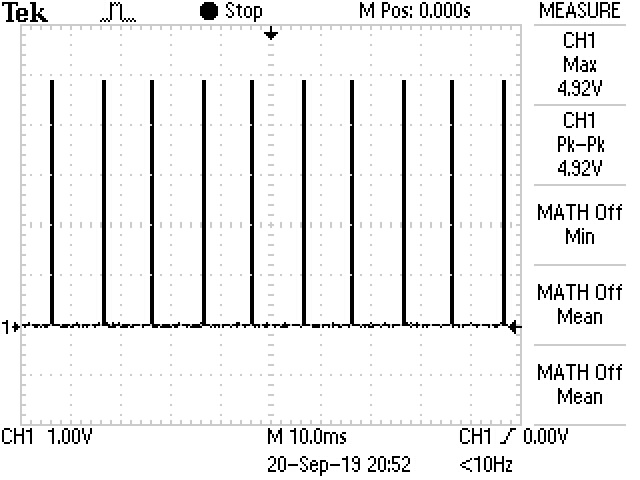
\includegraphics[width=1\linewidth]{./Figures/phasetransducermidrange.JPG}
    		    \caption{Mid range output for the phase transducer} \label{subfig:phaseshifttransducermidrange}
     \end{subfigure}
      \begin{subfigure}[]{0.45\textwidth}
      \centering
  		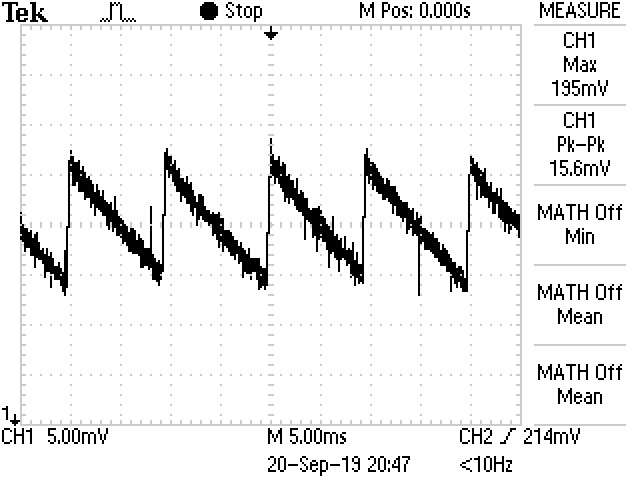
\includegraphics[width=1\linewidth]{./Figures/phasetransducernoise.JPG}
		    \caption{Ripple voltage after low pass filter} \label{subfig:phaseshifttransducerripple}
     \end{subfigure}
   \caption[Measured results for the phase transducer]{Output PWM signal and ripple voltage for the phase transducer. (a) depicts mid range output, (b) depicts voltage ripple after low pass filter. }
    \label{fig:simulation_results_box}
 \end{figure}
 




